

\section{Position Control of $n$ Robots Using Wall Friction}\label{sec:PostionControlnRobots}
%%%%%%%%%%%%%%%%%%%%%%%%%%%%%%%%%%%%%%%%%%%
Alg. \ref{alg:PosControl2Robots}  can be extended to control the position of $n$ robots using wall friction under several constraints. 
The solution described here is an iterative procedure with $n$ loops. 
 The $k$th loop moves the $k$th robot from a \emph{staging zone} to the desired position in a \emph{build zone}. 
  All robots move according to the global input, but due to wall friction, at the end the $k$th loop, robots 1 through $k$ are in their desired final configuration in the build zone, and robots $k+1$ to $n$ are in the staging zone. 
   See Fig.~\ref{fig:simulationNrobot} for a schematic of the build and staging zones.

\begin{figure}
\begin{center}
	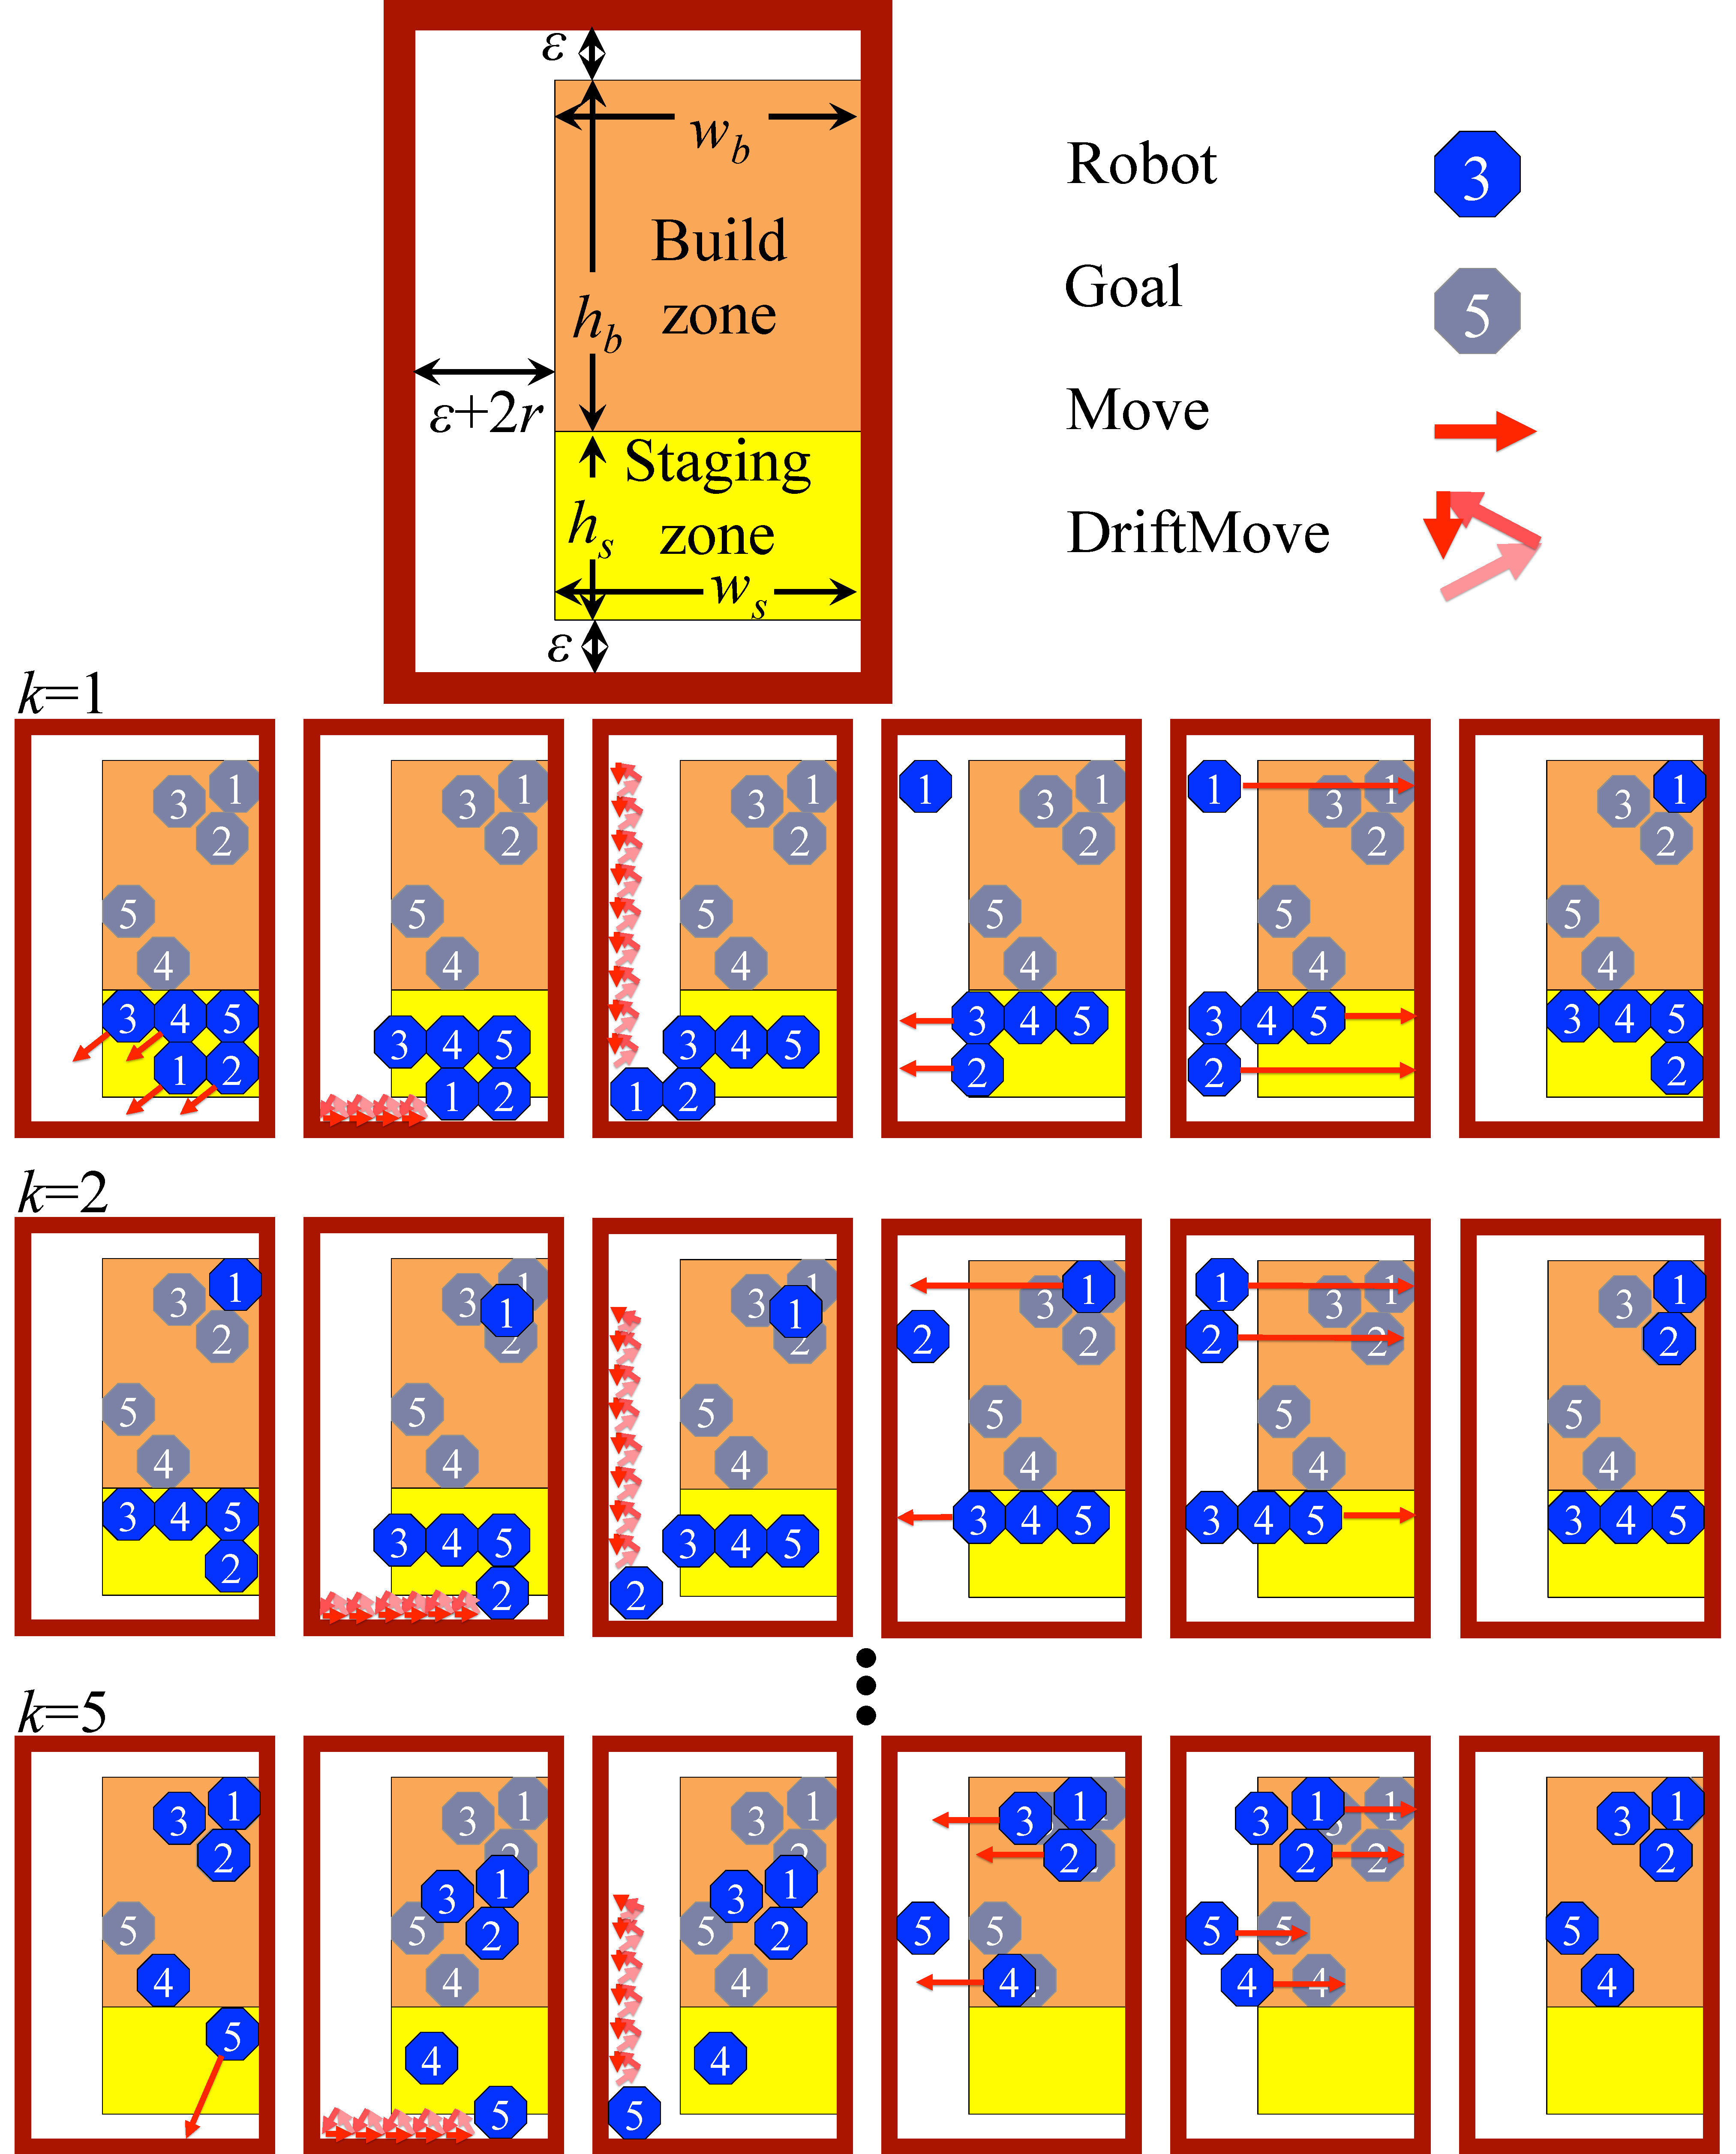
\includegraphics[width=1.0\columnwidth]{PositionNrobots.pdf}
\end{center}
\vspace{-1em}
\caption{\label{fig:simulationNrobot}
Illustration of Alg.\ \ref{alg:PosControlNRobots}, $n$ robot position control  using wall friction.
}
\end{figure}

Assume an open workspace with four axis-aligned walls with infinite friction.
The axis-aligned build zone of dimension $(w_b, h_b)$ containing the final configuration of $n$ robots must be disjoint from the axis-aligned staging zone of dimension $(w_s, h_s)$  containing the starting configuration of $n$ robots. Without loss of generality, assume the build zone  is above the staging zone. 
Furthermore, there must be at least $\epsilon$ space above the build zone, $\epsilon$ below the staging zone, and $\epsilon + 2r$ to the left of the build and staging zone, where $r$ is the radius of a robot.  The minimum workspace is then $(\epsilon + 2r + \max(w_b,w_s), 2\epsilon + h_s,h_b)$.

The $n$ robot position control algorithm relies on a $\text{\sc DriftMove}(\alpha, \beta, \epsilon,\theta)$ control input, described in Alg.~\ref{alg:DriftMove} and shown in Fig.\  \ref{fig:driftmove}.
For $\theta = 0^\circ$, a drift move consists of repeating a triangular movement sequence $\{ (\beta/2,-\epsilon),(\beta/2,\epsilon),(-\alpha,0)\}$. Any particle touching a top wall moves right $\beta$ units, while every particle not touching the top move right $\beta-\alpha$.

\begin{figure}
\begin{center}
%
\includegraphics[width=.47\columnwidth]{driftmove0.pdf}
%	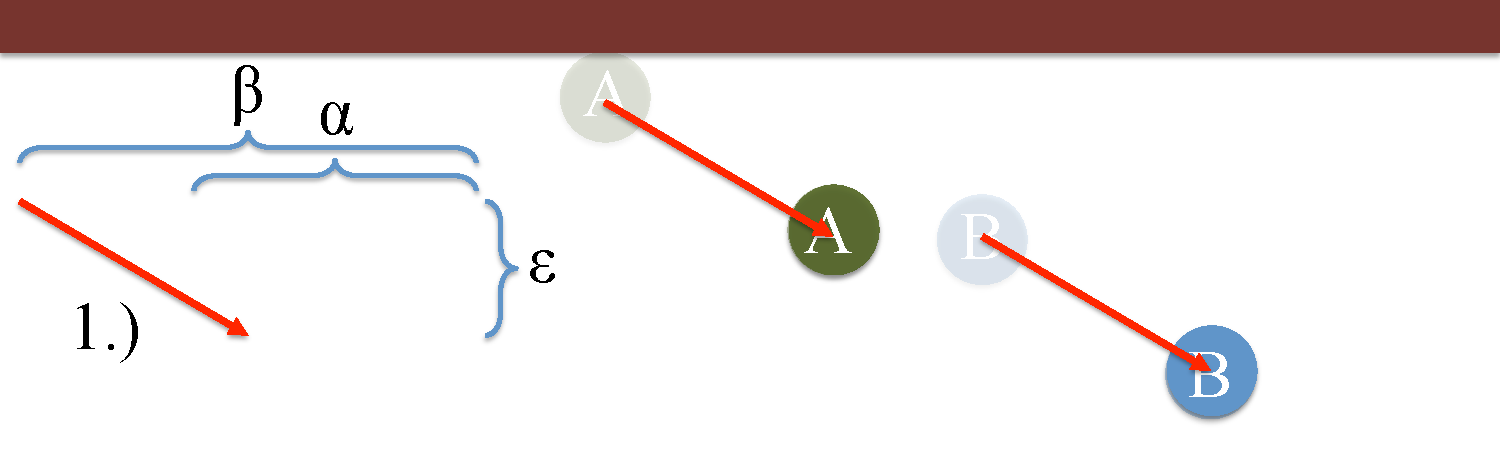
\includegraphics[width=.47\columnwidth]{driftmove1.pdf}
%	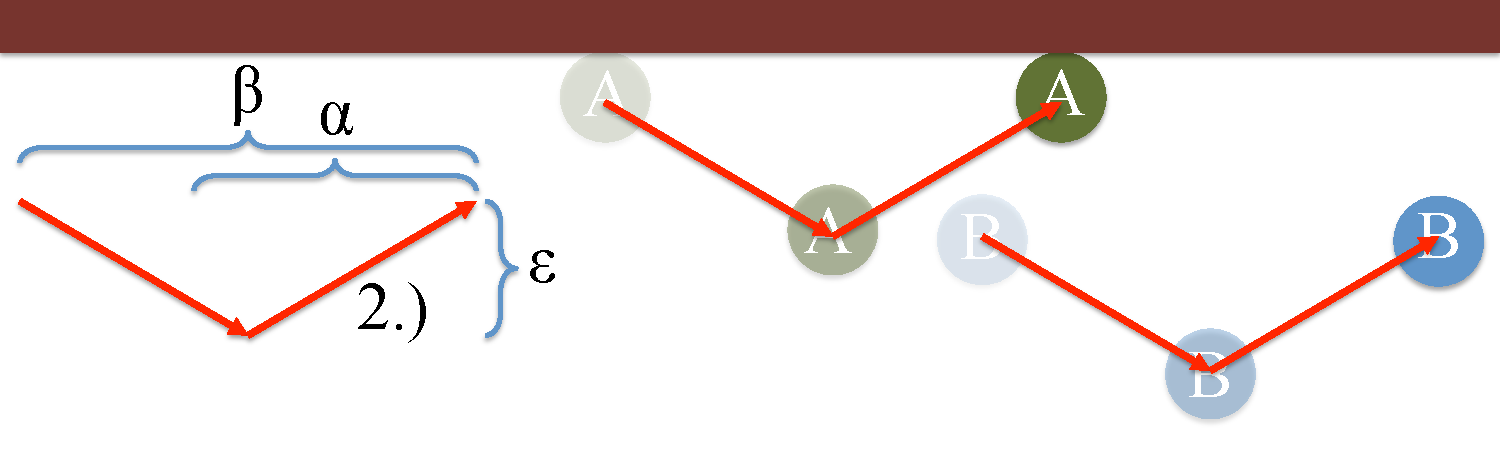
\includegraphics[width=.47\columnwidth]{driftmove2.pdf}
	\includegraphics[width=\columnwidth]{driftmovefullres.pdf}
\end{center}
\vspace{-1em}
\caption{\label{fig:driftmove}
A  $\text{\sc DriftMove}(\alpha, \beta, \epsilon,0^\circ)$ repeats a triangular movement sequence $\{ (\beta/2,-\epsilon),(\beta/2,\epsilon),(-\alpha,0)\}$. Robot $A$ touching a top wall moves right $\beta$ units, while robots not touching the top move right $\beta-\alpha$.}
\vspace{-1em}
\end{figure}

Let $(0,0)$ be the lower left corner of the workspace, $p_k$ the $x,y$ position of the $k$th robot, and $f_k$ the final $x,y$ position of the $k$th robot. Label the robots in the staging zone from left-to-right and bottom-to-top, and the $f_k$ configurations top-to-bottom and right-to-left as shown in Fig.~\ref{fig:construction2d}.

\begin{algorithm}
\caption{PositionControl$n$RobotsUsingWallFriction($k$)}\label{alg:PosControlNRobots}
\begin{algorithmic}[1]
\State Move( $-\epsilon, r-p_{ky}$) % move  away from right wall and down till robot k touches bottom


\While{ $p_{kx} > r$} 
\State $\text{\sc DriftMove}(\epsilon, \min(p_{kx} - r,\epsilon), \epsilon,180^\circ)$    %drift move left until kth robot touches left wall
\EndWhile

\State $m \gets \operatorname{ceil}(\frac{f_{ky}-r}{\epsilon})$
\State $\beta \gets \frac{f_{ky}-r}{m}$
\State $\alpha \gets \beta - \frac{r - p_{ky}-\epsilon}{m}$
\For{ $m$ iterations}
\State $\text{\sc DriftMove}(\alpha, \beta, \epsilon,90^\circ)$    %move kth robot to f_{ky} and leave the rest in position.
\EndFor

\State Move ($r+\epsilon-f_{kx}, 0$)  % move the group to the left until k is in the correct relative x position
\State Move ($f_{kx}-r, 0$)  

\end{algorithmic}
\end{algorithm}


\begin{algorithm}
\caption{ {\sc DriftMove}($\alpha,\beta,\epsilon,\theta$)
}\label{alg:DriftMove}
particles touching the wall move $\beta$ units, while particles not touching the wall move $\beta-\alpha$ units.
\begin{algorithmic}[1]
\State $R = \begin{bmatrix} \cos(\theta) & -\sin(\theta) \\
 \sin(\theta) & \cos(\theta)  \end{bmatrix}$
\State {\sc Move}$(R \cdot [\beta/2,-\epsilon]^\top)$ 
\State  {\sc Move}$(R \cdot [\beta/2,\epsilon]^\top)$ 
\State  {\sc Move}$(R \cdot [-\alpha,0]^\top)$ 
\end{algorithmic}
\end{algorithm}


Alg. \ref{alg:PosControlNRobots} proceeds as follows:  
First, the robots are moved left away from the right wall, and down so robot $k$ touches the bottom wall.
Second, a set of $\operatorname{DriftMove}$s are executed that move robot $k$ to the left wall with no net movement of the other robots.
Third, a set of $\operatorname{DriftMove}$s are executed that  move robot $k$ to its target height and return the other robots to their initial heights. 
Fourth, all robots except robot $k$ are pushed left until robot $k$ is in the correct relative $x$ position compared to robots 1 to $k-1$.
Finally, all robots are moved right until robot $k$ is in the desired target position. Running time is $O(n(w+h))$.



The hardware platform depicted in \ref{fig:construction2d} is an assembled practical setup that assumes that $\epsilon= 1$ cm. 
The workspace is a $7\times 7$ cm grid space. 
All particles are 3D-printed plastic whose top is a 1cm diameter cylinder with a narrower base that encapsulates a steel bearing ball.
Wall friction is emulated by a toothed wall design to keep particles from moving out of place while implementing the drift move. 
The workspace boundary is mounted on top of a white sheet of cardboard.
Underneath the cardboard, a grid of 3mm diameter magnets glued with 1 cm spacing to a thin board generates the global control input.
 A video attachment  shows the algorithm at work. 
This discretized setup requires several modification to Alg.~\ref{alg:PosControlNRobots}.
 In this demonstration, all moves are 1 cm in length.
   All drift moves are an counterclockwise \emph{square} move  of size 1 cm$\times$1 cm. 
   Once the $k$th roller gets to its designated location in each loop, a correction step is implemented. 
   This correction step increases by two the total number of moves required per particle.
   Fig.~\ref{fig:simulationNrobot} shows there are only 6 stages per particle involved in Alg.~\ref{alg:PosControlNRobots}.
The fixed step algorithm requires 8 stages per particle as shown in Fig.~\ref{fig:construction2d}. 

A significant difference between Alg.~\ref{alg:PosControlNRobots} and the fixed move implementation of it is that Alg.~\ref{alg:PosControlNRobots}
enables placing particles at arbitrary, non-overlapping locations, while the fixed move implementation requires goal locations at the center of grid cells. 

\begin{figure}
\begin{center}
	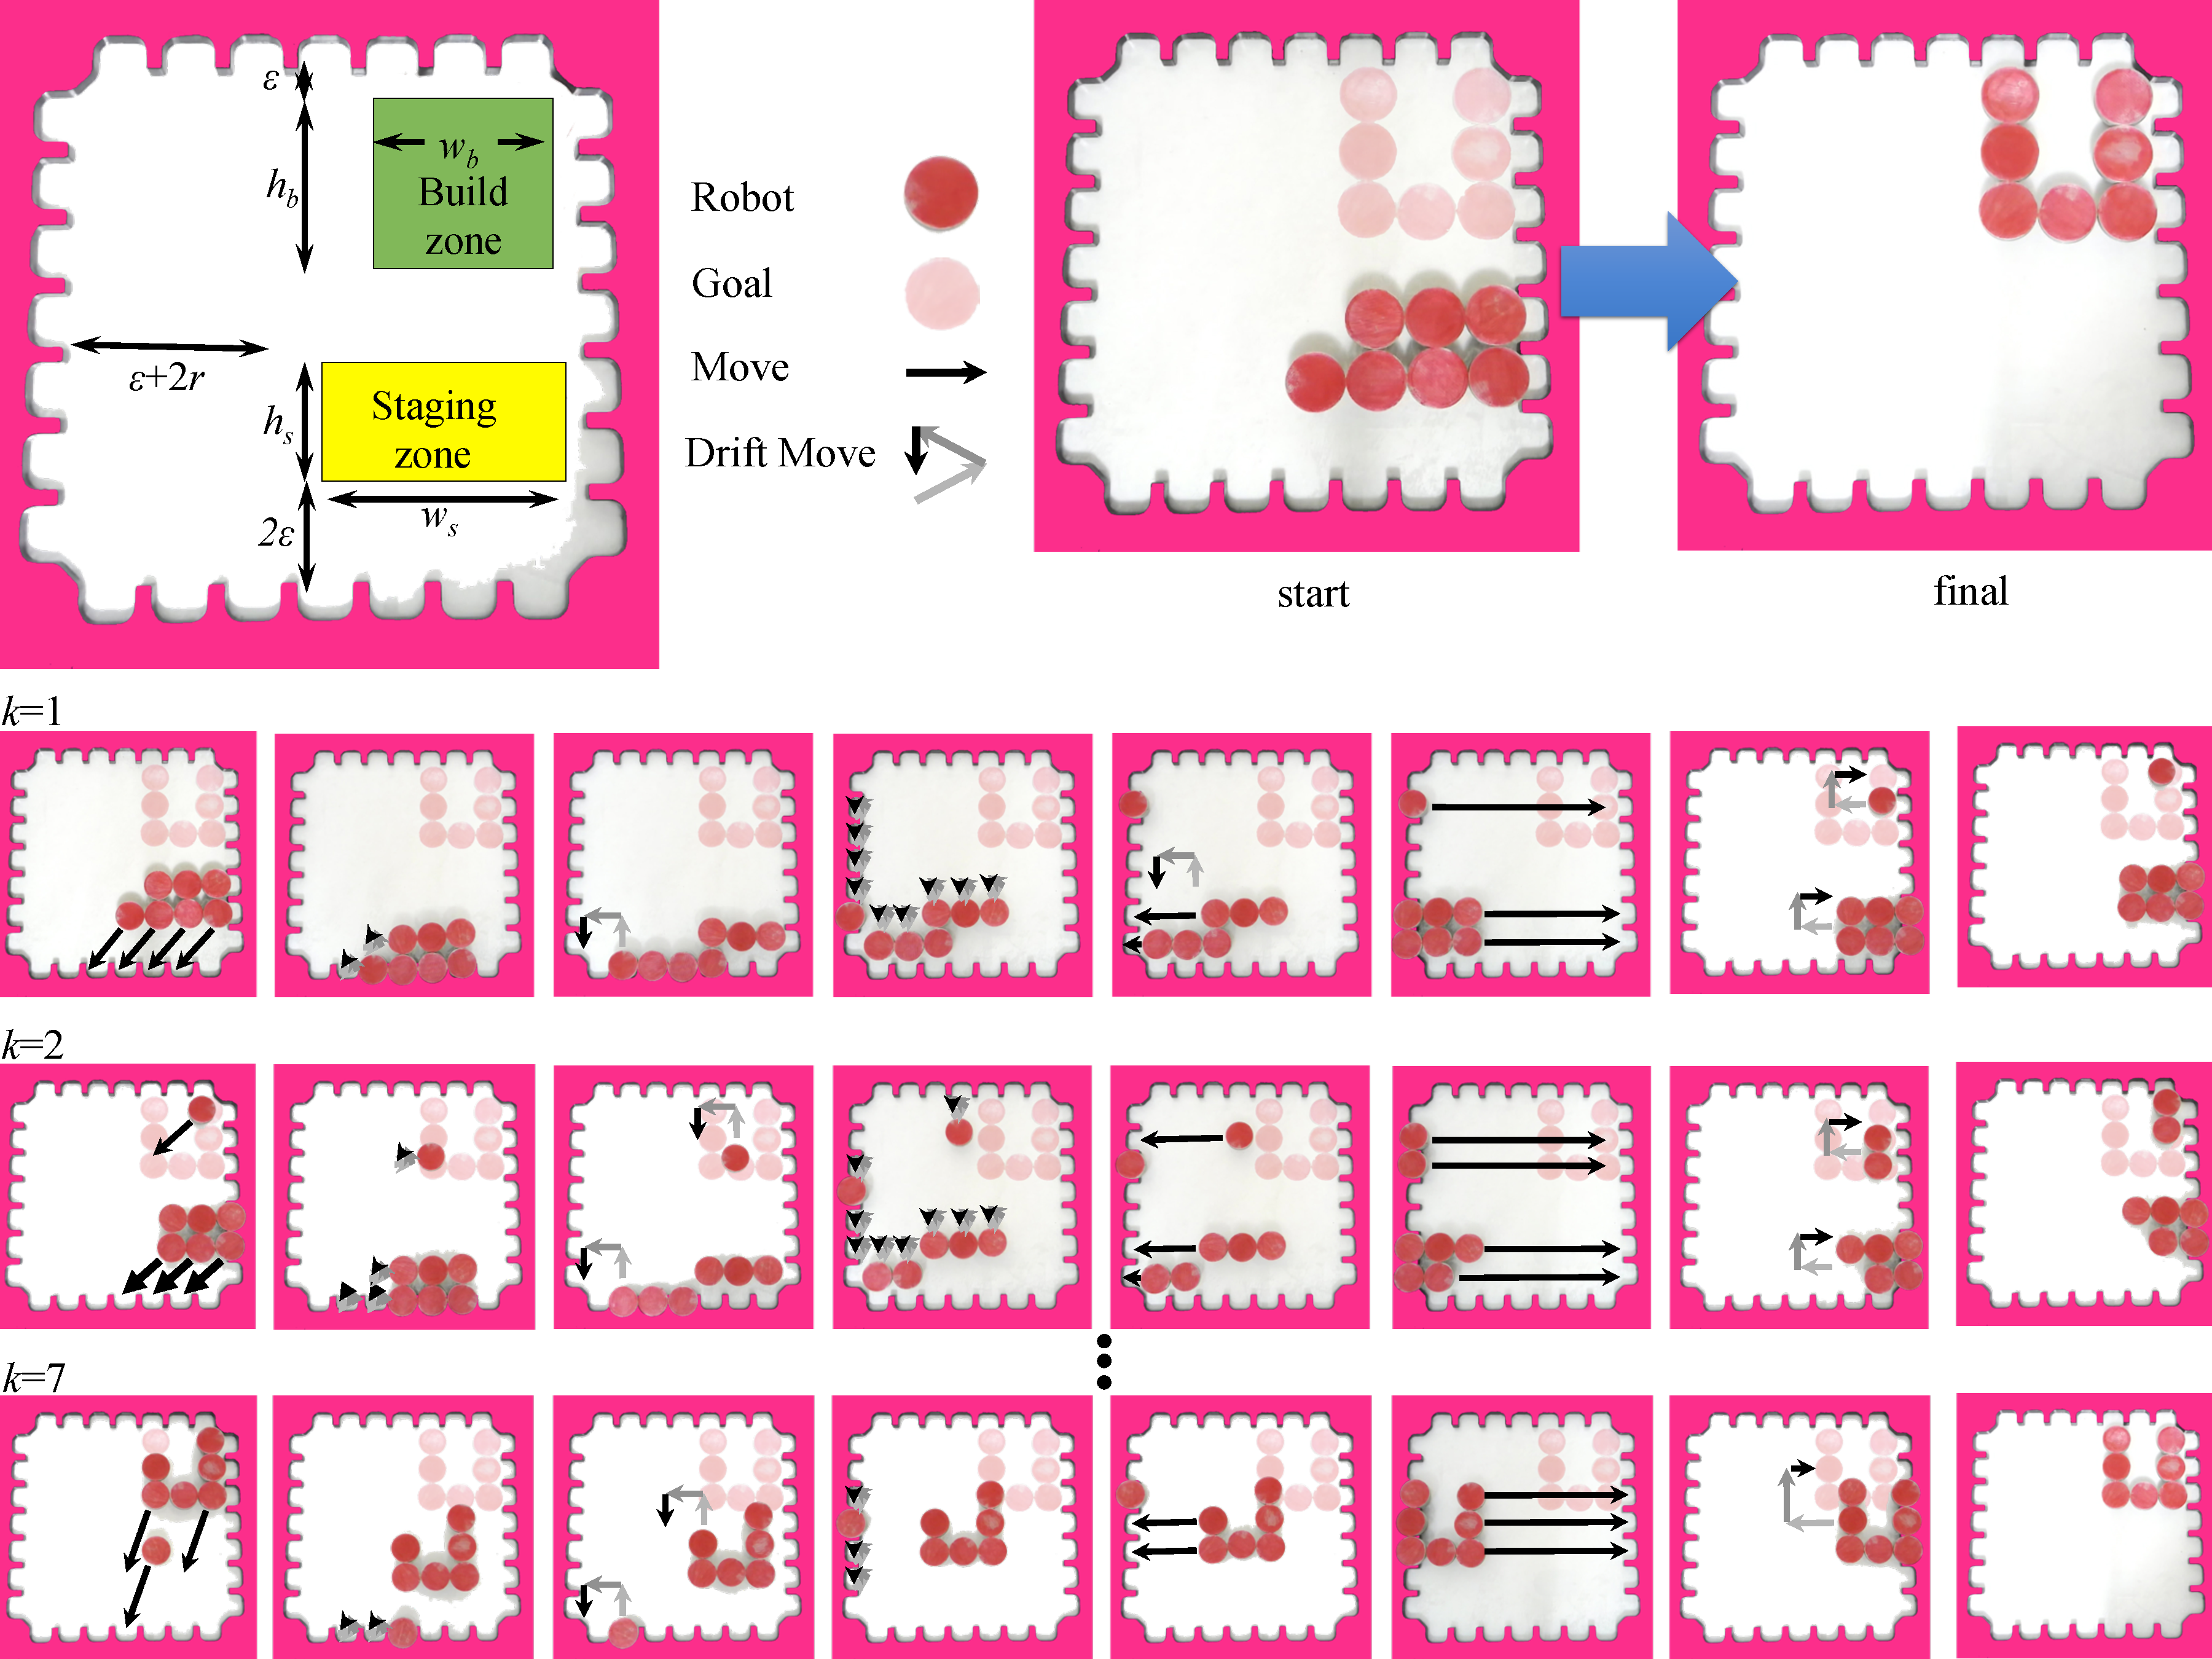
\includegraphics[width=1.0\columnwidth]{multirobotSliderHardware.pdf}
\end{center}
\vspace{-1em}
\caption{\label{fig:construction2d}
Illustration of Alg.\ \ref{alg:PosControlNRobots}, discretized $n$ robot position control  using wall friction.
}
\end{figure}

